% Copyright (c) 2025 Carl Martin Ludvig Sinander.

% This program is free software: you can redistribute it and/or modify
% it under the terms of the GNU General Public License as published by
% the Free Software Foundation, either version 3 of the License, or
% (at your option) any later version.

% This program is distributed in the hope that it will be useful,
% but WITHOUT ANY WARRANTY; without even the implied warranty of
% MERCHANTABILITY or FITNESS FOR A PARTICULAR PURPOSE. See the
% GNU General Public License for more details.

% You should have received a copy of the GNU General Public License
% along with this program. If not, see <https://www.gnu.org/licenses/>.

%%%%%%%%%%%%%%%%%%%%%%%%%%%%%%%%%%%%%%%%%%%%%%%%%%%%%%%%%%%%%%%%%%%%%%%

The project of this and the \hyperref[ch_osdp]{previous} chapter is to extend to dynamic games the tools of dynamic programming that are familiar from the analysis of single-agent dynamic decision problems: in particular, Blackwell's \emph{one-shot deviation principle} and the \emph{Bellman equation.} The previous chapter dealt with the one-shot deviation principle; in this chapter, we extend the Bellman equation.

We focus on the game-theoretic analogue of stationary single-agent dynamic decision problems: \emph{repeated games.} In particular, we study repeated games with public (possibly noisy) monitoring. The extension of the Bellman equation to such games is called `APS' after its originators, \textcite{AbreuPearceStacchetti1990}.



%%%%%%%%%%%%%%%%%%%%%%%%%%%%%%%%%%%
%%%%%%%%%%%%%%%%%%%%%%%%%%%%%%%%%%%
\section{Public-monitoring repeated games}
\label{aps:games}
%%%%%%%%%%%%%%%%%%%%%%%%%%%%%%%%%%%
%%%%%%%%%%%%%%%%%%%%%%%%%%%%%%%%%%%

\begin{definition}
	%
	\label{definition:stage_game}
	%
	A \emph{public-monitoring stage game} is a tuple $\left( I, Y, (A_i, u_i)_{i \in I}, \mu \right)$, where $I$ and $Y$ are non-empty sets, for each $i \in I$, $A_i$ is a non-empty set and $u_i$ is a function $A_i \times Y \to \R$, and $\mu$ is a function $A \to \Delta(Y)$.
	%
\end{definition}

The interpretation is that $I$ are players who simultaneously choose actions $a = (a_i)_{i \in I} \in \prod_{i \in I} A_i \equiv A$, whereupon a public \emph{outcome} $y \in Y$ is drawn from the probability distribution $\mu(\cdot|a) \in \Delta(Y)$. The payoff $u_i(a_i,y)$ of each player $i \in I$ depends on her own action $a_i \in A_i$ and on the public outcome $y \in Y$.

As usual, all players are assumed to have an expected-utility attitude to risk. We shall abuse notation by writing
%
\begin{equation}
	u_i(a)
	\coloneqq \E_{y \sim \mu(\cdot|a)}( u_i(a_i,y) )
	\label{eq:stage-game_normal}
\end{equation}
%
for the (expected) payoff of player $i \in I$ from action profile $a \in A$. As usual, we linearly extend each player~$i$'s payoff function $u_i$ to $\Delta(A)$: that is, for each mixed action profile $\alpha \in \Delta(A)$, we write $u_i(\alpha) \coloneqq \E_{a \sim \alpha}\left( u_i(a) \right)$. We similarly linearly extend $\mu$ by writing $\mu(y|\alpha) \coloneqq \E_{a \sim \alpha}\left( \mu(y|a) \right)$ for all $y \in Y$ and $\alpha \in \Delta(A)$.

On the one hand, obviously every normal-form game $\left( I, (A_i, u_i)_{i \in I} \right)$ is equivalent to the public-monitoring stage game $\left( I, Y, (A_i, u_i)_{i \in I}, \mu \right)$ in which $Y \coloneqq A$ and $\mu(a|a) = 1$ for every $a \in A$ (i.e. the `outcome' is simply the profile of actions played). But on the other hand, in light of the previous paragraph, every public-monitoring stage game $\left( I, Y, (A_i, u_i)_{i \in I}, \mu \right)$ is strategically equivalent to the normal-form game $\left( I, (A_i, u_i)_{i \in I} \right)$, where now each player~$i$'s payoff $u_i$ is a function of action profiles $a \in A$ (not action-and-outcome pairs $(a_i,y) \in A_i \times Y$), given by \cref{eq:stage-game_normal} above; nothing is lost in this reduction from a public-monitoring stage game to a normal-form game except the possibility that ex-post payoffs $(u_i(a))_{i \in I}$ are random conditional on the action profile $a \in A$ played, and such extrinsic randomness is strategically irrelevant (players only care about \emph{expected} payoffs and how these depend on action choice).

The point of the `public outcomes' formalism is to describe, when the game is played \emph{repeatedly,} what players know about their opponents' \emph{past} choices.

\begin{definition}
	%
	\label{definition:rep_game}
	%
	A \emph{public-monitoring repeated game} is a pair $(G,\delta)$, where $G = \left( I, Y, (A_i, u_i)_{i \in I}, \mu \right)$ is a public-monitoring stage game and $\delta \in (0,1)$.
	%
\end{definition}

The interpretation is that in each period $t \in \{0,1,2,3,\dots\}$, the public-monitoring stage game $G$ is played, meaning that the players simultaneously choose actions $a^t = \left(a_i^t\right)_{i \in I} \in A$, whereupon the public outcome $y^t \in Y$ is drawn from the probability distribution $\mu\left(\cdot\middle|a^t\right) \in \Delta(Y)$, generating stage-game payoffs $\left(u_i\left(a_i^t,y^t\right)\right)_{i \in I}$. Public outcomes are conditionally independent over time: that is, the public outcomes $y^t$ and $y^s$ in distinct periods $t \neq s$ are statistically independent conditional on the action profiles $a^t$ and $a^s$. The information available to each player $i \in I$ at the start of period $t \in \{0,1,2,3,\dots\}$ consists of her own past actions $\bigl( a_i^0, a_i^1, a_i^2, \dots, a_i^{t-1} \bigr) \in A_i^t$ and all past public outcomes $(y^0,y^1,y^2,\dots,y^{t-1}) \in Y^t$. The (total, lifetime) payoff of player $i \in I$ is the discounted mean of stage-game payoffs:
%
\begin{equation*}
	(1-\delta) \sum_{t=0}^\infty \delta^t u_i\left( a_i^t, y^t \right) .
\end{equation*}
%
(The normalisation by $1-\delta$ ensures that lifetime payoffs live in the same set $\{ u(\alpha) : \alpha \in \Delta(A) \}$ as stage-game payoffs; for example, earning a stage-game payoff of $x \in \R$ in every period yields a lifetime payoff of $(1-\delta) \frac{x}{1-\delta} = x$.)

Of course a public-monitoring repeated game is just one particular sort of extensive-form game, so can be described using the general formalism of extensive-form games; for completeness, we do this at the end of this section.

The pair $(Y,\mu)$ is called the game's \emph{monitoring technology,} since it describes how players learn about the past actions taken by their opponents. The \emph{perfect monitoring structure} is the monitoring structure $(Y,\mu)$ given by $Y \coloneqq A$ and $\mu(a|a) \coloneqq 1$ for every $a \in A$.

\begin{example}
	%
	\label{example:rep_pris}
	%
	Recall the prisoner's dilemma (\cpageref{example:prisoners} above): players $I=\{1,2\}$, actions $A_1=A_2=\{C,D\}$ and payoffs
	%
	\begin{equation*}
		\begin{array}{c|cc}
			  & C   & D   \\ \hline
			C & 2,2 & 0,3 \\
			D & 3,0 & 1,1
		\end{array} 
	\end{equation*}
	%
	Consider the \emph{repeated prisoners' dilemma,} in which the prisoners' dilemma is played repeatedly with perfect monitoring and a discount factor $\delta \in (0,1)$. It is a public-monitoring repeated game. Are there equilibria in which players always play the cooperative action $C$ (which is strictly dominated in the stage game)? (Yes if $\delta \geq 1/2$, as we shall show in \cref{aps:examples:rep_pris_gen} below.)
	%
\end{example}

\begin{example}
	%
	\label{example:greenporter}
	%
	Consider the Green--Porter (\citeyear{GreenPorter1984}) model of tacit collusion in oligopoly. This is the public-monitoring repeated game whose stage game is a noisy version of the \textcite{Cournot1838} model from \Cref{example:cournot} (\cref{dom:rbty}, \cpageref{example:cournot}): each of two firms $i \in I \coloneqq \{1,2\}$ simultaneously chooses what quantity $a_i \in A_i \coloneqq \R_+$ to produce, earning profit $u_i\left(a_i,y\right) \coloneqq a_i \times (y - c)$ where $c>0$, and where $y \coloneqq \kappa - \lambda(a_1+a_2)$ for some random variables $\kappa$ and $\lambda$ that satisfy $\kappa > c > 0 < \lambda$ a.s.
	(So the monitoring technology is $((0,\infty),\mu)$ where for each $(a_1,a_2) = a \in A$, $\mu(\cdot|a)$ denotes the CDF of the random variable $\kappa - \lambda(a_1+a_2)$. Assume for simplicity that this CDF has full support.) The interpretation is that marginal cost is $c$ and that the market price $y$ is determined by the noisy inverse market demand curve $q \mapsto \kappa - \lambda q$.

	Recall that in the unique rationalisable outcome of the stage game, both firms produce $\left[\E(\kappa)-c\right]/3\E(\lambda)$, earning expected profits of $\pi^\star \coloneqq \left[\E(\kappa)-c\right]^2 / 9 \E(\lambda)$. In the repeated game, are there \emph{(tacitly) collusive equilibria,} meaning equilibria in which both firms' expected discounted mean payoffs strictly exceed $\pi^\star$? (Yes if $\delta$ is large enough, as we shall see in \cref{aps:examples:greenporter_gen} below.)
	%
\end{example}

\begin{example}
	%
	\label{example:sovereign}
	%
	Sovereign debt (loans to states/governments) differs from other debt in that sovereigns are, well, sovereign: they cannot be compelled to keep their promises, so repayment is always voluntary. So why do sovereigns ever repay their debts instead of defaulting? This question is the starting point of a rich literature in macroeconomics \parencite[see][]{AguiarAmador2021}.%
		\footnote{There are several reasons why this question is important. For example, a sovereign who is expected to default is unlikely to obtain much credit in the first place, and sovereign access to credit matters enormously for the ability to wage war: classic examples are the Eighty Years' War and the Second Hundred Years' War, in both of which the victor was much smaller but had far better access to credit.}
	A (the?) natural answer is that creditors may be able to deter default by credibly threatening exclusion from \emph{future} borrowing.

	To formalise this story parsimoniously, consider the \emph{extensive-form} stage game in \Cref{fig:sov}, in which a creditor chooses whether or not to lend £1 to a sovereign at interest rate $r>0$ to fund a project with net return $\pi>r$, and in case the loan was made, the sovereign then decides whether to repay it or default.
	%
	\begin{figure}
		\centering
		\usetikzlibrary{trees, arrows.meta, positioning}
		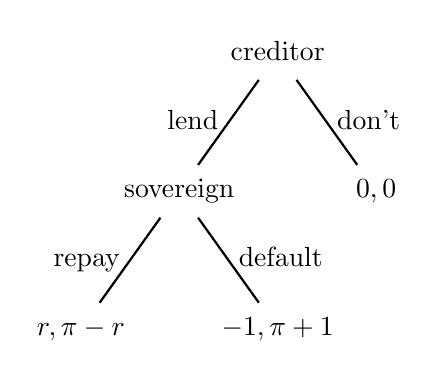
\begin{tikzpicture}[
			edge from parent/.style={thick, draw, font=\normalsize},
			decision/.style={font=\normalsize},
			terminal/.style={font=\normalsize},
			sibling distance=2.5cm,
			level distance=1.75cm
			]
			\node[decision] (creditor) {creditor\strut}
				child { node[decision] (sovereign) {sovereign\strut}
					child { node[terminal] {$r,\pi - r$\strut} edge from parent node[midway, left] {repay\strut} }
					child { node[terminal] {$-1,\pi + 1$\strut} edge from parent node[midway, right] {default\strut} }
					edge from parent node[midway, left] {lend\strut}
					}
				child { node[terminal] {$0,0$\strut} edge from parent node[midway, right] {don't\strut} };
		\end{tikzpicture}
		\caption{The stage game in \Cref{example:sovereign}.}
		\label{fig:sov}
	\end{figure}
	%
	Formally, this is the public-monitoring stage game $G = \left( I, Y, (A_i, u_i)_{i \in I}, \mu \right)$ with players $I \coloneqq \{\text{c(reditor)},\text{s(overeign)}\}$, actions $A_{\text{c}} \coloneqq \{\text{lend},\text{don't}\}$ and $A_{\text{s}} \coloneqq \{\text{repay},\text{default}\}$, monitoring structure $(Y,\mu)$ where $Y \coloneqq \text\{ \text{don't}, (\text{lend},\text{repay}), (\text{lend},\text{default}) \}$ and 
	%
	\begin{align*}
		\mu(\text{don't}|(\text{don't},\text{repay}))
		&\coloneqq 1 ,
		\\
		\mu(\text{don't}|(\text{don't},\text{default}))
		&\coloneqq 1 ,
		\\
		\mu((\text{lend},\text{repay})|(\text{lend},\text{repay}))
		&\coloneqq 1
		\quad \text{and}
		\\
		\mu((\text{lend},\text{default})|(\text{lend},\text{default}))
		&\coloneqq 1 ,
	\end{align*}
	%
	and payoffs
	%
	\begin{equation*}
		\left( u_{\text{c}}(a_{\text{c}},y) ,
		u_{\text{s}}(a_{\text{s}},y) \right)
		\coloneqq
		\begin{cases}
			(0,0) & \text{if $y = \text{don't}$} \\
			(r,\pi - r) & \text{if $y = (\text{lend},\text{repay})$} \\
			(-1,\pi + 1) & \text{if $y = (\text{lend},\text{default})$.}
		\end{cases}
	\end{equation*}

	Evidently the unique subgame-perfect equilibrium of the stage game $G$ is $(\text{don't},\text{default})$, which is Pareto-dominated by the strategy profile $(\text{lend},\text{repay})$ since $\pi > r > 0$. Are there equilibria of the \emph{repeated} game $(G,\delta)$ in which $(\text{lend},\text{repay})$ is played in every period on the path? (Yes if $\delta \geq (1+r)/(1+\pi)$, as we shall show in \cref{aps:examples:sovereign_gen} below.)
	%
\end{example}

What makes public monitoring `public' is that it is always commonly known what players know about other players' past actions: everyone observes $y \in Y$ and nothing else, everyone knows that everyone observes $y \in Y$ and nothing else, everyone knows that everyone knows that everyone observes $y \in Y$ and nothing else, and so on. This `publicness' property is built in to the definition of a public-monitoring repeated game. One can consider a more general type of repeated game in which players may observe \emph{private} signals which are informative about other players' past actions; these are called \emph{private-monitoring repeated games.} An example is if player~1 \emph{privately} observes the realisation of a noisy signal that is informative about player~2's last action, so that player~2 and player~3 do not know what player~1 knows (or believes) about player~2's last action. Private monitoring is arguably natural in many economic applications, but it is much less tractable than the public-monitoring case, and thus beyond the scope of this chapter. See \textcite[][chapters~12--14]{MailathSamuelson2006} if you're curious.

The definitions above of public-monitoring stage and repeated games omit some measure-theoretic niceties. We will sweep all such unpleasantness under the rug by focussing on \emph{finite} games. A public-monitoring stage game $G = \left( I, Y, (A_i, u_i)_{i \in I}, \mu \right)$ is called \emph{finite} iff the sets $I$, $Y$ and $(A_i)_{i \in I}$ are all finite. A public-monitoring repeated game $(G,\delta)$ is called \emph{finite} iff the public-monitoring stage game $G$ is finite. Our focus on finite games is for simplicity only; all of the results in this chapter do extend to infinite games \parencite[see][chapter~7]{MailathSamuelson2006}.

\begin{remark}
	%
	\label{remark:rep_game_formal}
	%
	As mentioned above, for a finite public-information stage game $G = \left( I, Y, (A_i, u_i)_{i \in I}, \mu \right)$ and a $\delta \in (0,1)$, the public-monitoring repeated game $(G,\delta)$ is formally an extensive-form game, namely
	%
	\begin{equation*}
		\left(\widetilde{I},\widetilde{\mathcal{A}},\widetilde{H},\widetilde{P},\widetilde{A},\widetilde{\mathcal{S}},\left(\widetilde{u}_i\right)_{i \in I},\widetilde{\pi}\right)
	\end{equation*}
	%
	where
	%
	\begin{itemize}
	
		\item the players are $\widetilde{I} \coloneqq I$,
		
		\item the actions are $\widetilde{\mathcal{A}} \coloneqq \left( \bigcup_{i \in I} A_i \right) \cup Y$,

		\item the histories $\widetilde{H}$ are all sequences $h$ in $\widetilde{\mathcal{A}}$ (including the empty sequence) such that for each $k \in \N$, the $k^\text{th}$ entry of $h$

		\begin{itemize}
		
			\item belongs to $A_1$ if $k = (\abs*{I}+1) n + 1$ for some $n \in \{0,1,2,3,\dots\}$,

			\item belongs to $A_2$ if $k = (\abs*{I}+1) n + 2$ for some $n \in \{0,1,2,3,\dots\}$,

			\item[\vdots]

			\item belongs to $A_{\abs*{I}}$ if $k = (\abs*{I}+1) n + \abs*{I}$ for some $n \in \{0,1,2,3,\dots\}$, and

			\item belongs to $Y$ if $k = (\abs*{I}+1) (n+1)$ for some $n \in \{0,1,2,3,\dots\}$,
		
		\end{itemize}
		%
		(where the non-terminal histories are the finite ones, and the terminal histories are the infinite ones,)

		\item the player and action functions $\widetilde{P}$ and $\widetilde{A}$ are given by

		\begin{itemize}
		
			\item $\widetilde{P}(h) \coloneqq 1$ and $\widetilde{A}(h) \coloneqq A_1$ if $\text{length}(h) = (\abs*{I}+1) n$ for some $n \in \{0,1,2,3,\dots\}$,
		
			\item $\widetilde{P}(h) \coloneqq 2$ and $\widetilde{A}(h) \coloneqq A_2$ if $\text{length}(h) = (\abs*{I}+1) n + 1$ for some $n \in \{0,1,2,3,\dots\}$,

			\item[\vdots]

			\item $\widetilde{P}(h) \coloneqq \abs*{I}$ and $\widetilde{A}(h) \coloneqq A_{\abs*{I}}$ if $\text{length}(h) = (\abs*{I}+1) n + \abs*{I}-1$ for some $n \in \{0,1,2,3,\dots\}$, and

			\item $\widetilde{P}(h) \coloneqq \text{Nature}$ and $\widetilde{A}(h) \coloneqq Y$ if $\text{length}(h) = (\abs*{I}+1) n + \abs*{I}$ for some $n \in \{0,1,2,3,\dots\}$,
		
		\end{itemize}

		\item the information sets $\widetilde{\mathcal{S}}$ are, for each non-terminal (meaning \emph{finite}) history $h \in \widetilde{H}$,

		\begin{itemize}
		
			\item if $\widetilde{P}(h) = i \in I$, then the information set $\widetilde{\mathcal{S}}(h)$ comprises all non-terminal histories $h'$ such for every $n \in \{0,1,2,3,\dots\}$, the $[(\abs*{I}+1) n + i]^\text{th}$ and $[(\abs*{I}+1) (n+1)]^\text{th}$ entries of $h$ and $h'$ (if there are such entries) are equal, and

			\item if $\widetilde{P}(h) = \text{Nature}$, then $\widetilde{\mathcal{S}}(h) \coloneqq \{h\}$,
		
		\end{itemize}

		\item the payoff functions $\left(\widetilde{u}_i\right)_{i \in I}$ are given by, for each terminal (meaning \emph{infinite}) history
		%
		\begin{equation*}
			h = \left(a_1^1,a_2^1,\dots,a_{\abs*{I}}^1,y^1,a_1^2,a_2^2,\dots,a_{\abs*{I}}^2,y^2,a_1^3,a_2^3,\dots,a_{\abs*{I}}^3,y^3,\dots\right) \in \widetilde{H} ,
		\end{equation*}
		%
		and each player $i \in I$,
		%
		\begin{equation*}
			\widetilde{u}_i(h) \coloneqq (1-\delta) \sum_{t=0}^\infty \delta^t u_i(a_i^t,y^t) ,
		\end{equation*}
		%
		and

		\item the Nature strategy function $\widetilde{\pi}$ is given by, for each non-terminal (meaning \emph{finite}) history
		%
		\begin{multline*}
			h = \Bigl(
			a_1^1,a_2^1,\dots,a_{\abs*{I}}^1,y^1,
			a_1^2,a_2^2,\dots,a_{\abs*{I}}^2,y^2,\dots,\\
			a_1^{t-1},a_2^{t-1},\dots,a_{\abs*{I}}^{t-1},y^{t-1},
			a_1^t,a_2^t,\dots,a_{\abs*{I}}^t\Bigr) \in \widetilde{H} 
		\end{multline*}
		%
		such that $\widetilde{P}(h)=\text{Nature}$,
		%
		\begin{equation*}
			\widetilde{\pi}(h) \coloneqq \mu\left(\cdot\middle|a_1^t,a_2^t,\dots,a_{\abs*{I}}^t\right) \in \Delta(Y) .
		\end{equation*}

	\end{itemize}
	%
\end{remark}




%%%%%%%%%%%%%%%%%%%%%%%%%%%%%%%%%%%
%%%%%%%%%%%%%%%%%%%%%%%%%%%%%%%%%%%
\section{Histories, strategies, payoffs}
\label{aps:hist}
%%%%%%%%%%%%%%%%%%%%%%%%%%%%%%%%%%%
%%%%%%%%%%%%%%%%%%%%%%%%%%%%%%%%%%%

For any non-empty set $X$ and $t \in \N$, recall that $X^t$ denotes the set of length-$t$ sequences in $X$, i.e.
%
\begin{equation*}
	X^t
	\coloneqq \left\{ \left( x^0, x^1, x^2, \dots, x^{t-1} \right) : x^0 \in X,\, x^1 \in X,\, x^2 \in X, \dots,\, x^{t-1} \in X \right\} .
\end{equation*}
%
There is of course only one length-$0$ sequence in $X$, namely the empty sequence, which we denote by $\varnothing$; for this reason, we write $X^0 \coloneqq \{\varnothing\}$.

Fix a finite public-monitoring repeated game
%
\begin{equation*}
	(G,\delta) = \left( I, Y, (A_i, u_i)_{i \in I}, \mu, \delta \right) .
\end{equation*}
%
At the start of each period $t \in \{0,1,2,3,\dots\}$, there is a \emph{public history}
%
\begin{equation*}
	h^{t-1} \equiv \left(y^0,y^1,y^2,\dots,y^{t-1}\right) \in Y^t
\end{equation*}
%
observed by all players and, for each player $i \in I$, a \emph{private history}
%
\begin{equation*}
	h^{t-1}_i \equiv \left(y^0,a^0_i,y^1,a^1_i,y^2,a^2_i,\dots,y^{t-1},a^{t-1}_i\right) \in (Y \times A_i)^t
\end{equation*}
%
observed only by player~$i$.

A \emph{(behavioural) strategy} of player $i \in I$ is a map $\sigma_i : \Union_{t=0}^\infty (Y \times A_i)^t \to \Delta(A_i)$ which specifies a (mixed) action at each private history of player~$i$. A (behavioural) strategy $\sigma_i$ of player $i \in I$ is called \emph{public} iff it is measurable with respect to the public history, i.e. there exists a function $\tau_i : \Union_{t=0}^\infty Y^t \to \Delta(A_i)$ such that
%
\begin{equation*}
	\sigma_i\left(y^0,a^0_i,y^1,a^1_i,y^2,a^2_i,\dots,y^{t-1},a^{t-1}_i\right)
	= \tau_i\left( y^0, y^1, y^2, \dots, y^{t-1} \right)
\end{equation*}
%
for every private history
%
\begin{equation*}
	\left(y^0,a^0_i,y^1,a^1_i,y^2,a^2_i,\dots,y^{t-1},a^{t-1}_i\right)
	\in (Y \times A_i)^t .
\end{equation*}
%
A \emph{(public) strategy profile} is a collection $\sigma = (\sigma_i)_{i \in I}$ of (public) strategies, one for each player. For a public strategy profile $\sigma$, we abuse notation by writing $\sigma\bigl(h^{t-1}\bigr) \in \prod_{i \in I} \Delta(A_i)$ for the mixed action profile played at public history $h^{t-1} \in Y^t$. (Why is this an abuse of notation?)

Any public strategy profile $\sigma$ generates, for each $t \in \{0,1,2,3,\dots\}$, a random length-$t$ public history $h^{t-1}_\sigma \in Y^t$: in particular, $h^{-1}_\sigma \coloneqq \varnothing$ (the empty sequence), $h^0_\sigma \coloneqq (y^0_\sigma)$ where $y^0_\sigma$ is drawn from $\mu\left( \cdot \middle| \sigma\left( h^{-1}_\sigma \right) \right)$, $h^1_\sigma \coloneqq \left(h^0_\sigma,y^1_\sigma\right)$ where $y^1_\sigma$ is drawn from $\mu\left( \cdot \middle| \sigma\left( h^0_\sigma \right) \right)$, $h^2_\sigma \coloneqq \left(h^1_\sigma,y^2_\sigma\right)$ where $y^2_\sigma$ is drawn from $\mu\left( \cdot \middle| \sigma\left( h^1_\sigma \right) \right)$, and so on, where the draws are jointly independent. The (lifetime) expected payoff of player $i \in I$ from the strategy profile $\sigma$ is denoted
%
\begin{equation*}
	U_i(\sigma) \coloneqq (1-\delta) \sum_{t=0}^\infty \delta^t u_i\left( \sigma\left(h^{t-1}_\sigma\right) \right) .
\end{equation*}
%
We write $U(\sigma) \coloneqq (U_i(\sigma))_{i \in I}$ for the vector of all players' lifetime payoffs. Similarly, we write $u(\alpha) \coloneqq (u_i(\alpha))_{i \in I}$ for the vector of all players' stage-game payoffs from a mixed action profile $\alpha \in \prod_{i \in I} \Delta(A_i)$.

Although the `continuation game' starting from a public history $h^{t-1} \in Y^t$ is \emph{not} a subgame (except if monitoring is perfect), it can still be treated as a game in its own right \emph{provided} players play a public strategy profile, since then players' private information about their own past play is irrelevant for payoffs going forward. By inspection, this `continuation game' is identical with the full public-monitoring repeated game $(G,\delta)$ itself: the game is $G$ is played repeatedly, with public outcomes drawn conditionally independently over time, and payoffs discounted by $\delta$.

Given a public strategy profile $\sigma$ and a public history $h_{*}^{t-1} \in Y^t$, the \emph{continuation strategy profile} is the strategy profile $\sigma|_{h_{*}^{t-1}}$ defined by
%
\begin{equation*}
	\left.\sigma\right|_{h_{*}^{t-1}}\left( h^{s-1} \right)
	\coloneqq \sigma\left( h_{*}^{t-1}, h^{s-1} \right)
	\quad \text{for each public history $h^{s-1} \in Y^s$.}
\end{equation*}
%
To be very clear about notation here: $(h_{*}^{t-1}, h^{s-1}) \in Y^{t+s}$ is the sequence in $Y$ obtained by concatenating the sequences $h_{*}^{t-1} \in Y^t$ and $h^{s-1} \in Y^s$. In other words, $(h_{*}^{t-1}, h^{s-1})$ is the length-$(t+s)$ public history in which public outcomes are $h_{*}^{t-1}$ in periods $\{0,1,2,3,\dots,t-2,t-1\}$ and $h^{s-1}$ in periods $\{t,t+1,t+2,t+3,\dots,t+s-2,t+s-1\}$.

Obviously every continuation of a public strategy profile is itself public. For each player $i \in I$, we write $\sigma_i|_{h^{t-1}} \coloneqq \left( \sigma|_{h^{t-1}} \right)_i$ for $i$'s continuation strategy and $\sigma_{-i}|_{h^{t-1}} \coloneqq \left( \sigma|_{h^{t-1}} \right)_{-i}$ for the profile of continuation strategies of her opponents.

The \emph{continuation payoff} of a public strategy profile $\sigma$ at a public history $h_{*}^{t-1} \in Y^t$ is the payoff from play of the (public) continuation strategy profile $\sigma_{*} \coloneqq \sigma|_{h_{*}^{t-1}}$ in the `continuation game' that starts at $h_{*}^{t-1}$, i.e.
%
\begin{align*}
	U\left( \sigma_{*} \right)
	&= (1-\delta) \sum_{s=0}^\infty \delta^s u\left( \sigma_{*}\left(h^{s-1}_{\sigma_{*}}\right) \right)
	\\
	&= (1-\delta) \sum_{s=t}^\infty \delta^{s-t} u\left( \sigma\left(h_{*}^{t-1},h^{s-t-1}_{\sigma_{*}} \right) \right) .
\end{align*}
%
Note that by definition, the continuation payoff from public history $h_{*}^{t-1} \in Y^t$ omits per-period payoffs enjoyed in periods $\{0,1,2,3,\dots,t-1\}$; it is a forward-looking object.

Continuation payoffs of public strategy profiles have a recursive structure: for any public strategy profile $\sigma$ and public history $h^{t-1} \in Y^t$,
%
\begin{equation*}
	U\left(\sigma|_{h^{t-1}}\right)
	= (1-\delta) u\left( \sigma\left( h^{t-1} \right) \right)
	+ \delta \E\left( U\left( \sigma|_{\left( h^{t-1}, y^t \right)} \right) \right),
\end{equation*}
%
where $y^t$ is a random draw from the distribution $\mu\left( \cdot \middle| \sigma\left( h^{t-1} \right) \right)$; in other words,
%
\begin{equation*}
	U\left(\sigma|_{h^{t-1}}\right)
	= (1-\delta) u\left( \sigma\left( h^{t-1} \right) \right)
	+ \delta \sum_{y \in Y}
	U\left( \sigma|_{\left( h^{t-1}, y \right)} \right)
	\mu\left( y \middle| \sigma\left( h^{t-1} \right) \right) .
\end{equation*}



%%%%%%%%%%%%%%%%%%%%%%%%%%%%%%%%%%%
%%%%%%%%%%%%%%%%%%%%%%%%%%%%%%%%%%%
\section{Perfect public equilibrium}
\label{aps:ppe}
%%%%%%%%%%%%%%%%%%%%%%%%%%%%%%%%%%%
%%%%%%%%%%%%%%%%%%%%%%%%%%%%%%%%%%%

Again fix a finite public-monitoring repeated game
%
\begin{equation*}
	(G,\delta) = \left( I, Y, (A_i, u_i)_{i \in I}, \mu, \delta \right) .
\end{equation*}
%
A player~$i$ may sometimes strictly prefer a non-public strategy over all public strategies. In particular, if ($i$ believes that) a player $j \neq i$ is playing a non-public strategy, then player~$j$'s actions today depend on what actions she took in the past, which only she knows. To predict player~$j$'s choice of action, player~$i$ must guess player~$j$'s past actions based on past public outcomes. The distribution of these outcomes depend both on her own past actions and on those of player~$j$. Thus to draw correct inferences about what actions player~$j$ likely took in the past, player~$i$ must in general make use of her knowledge of her \emph{own} past actions. When choosing her action based on a belief formed in this way, player~$i$'s action may well depend on what actions she herself took in previous periods. In other words, she may wish to use a non-public strategy.

However, if (player~$i$ believes that) the other players play \emph{public} strategies, then she always has a public best reply:

\begin{observation}
	%
	\label{observation:public_br}
	%
	Fix a finite public-monitoring repeated game
	%
	\begin{equation*}
		(G,\delta) = \left( I, Y, (A_i, u_i)_{i \in I}, \mu, \delta \right) ,
	\end{equation*}
	%
	a player $i \in I$, a public history $h^{t-1} \in Y^t$, and strategies $\sigma_j : \Union_{t=0}^\infty (Y \times A_j)^t \to \Delta(A_j)$ of each other player $j \in I \setminus \{i\}$. If $\sigma_j$ is public for each $j \in I \setminus \{i\}$, then $i$ has a public best reply at $h^{t-1}$: that is, there is a public strategy $\sigma_i$ of player~$i$ such that
	%
	\begin{equation*}
		U_i\left( \sigma|_{h^{t-1}} \right) \geq U_i\left( \sigma_i', \sigma_{-i}|_{h^{t-1}} \right)
	\end{equation*}
	%
	for every strategy $\sigma_i'$ of player~$i$.
	%
\end{observation}

This is (nearly) obvious upon reflection: player~$i$'s past actions are not directly payoff-relevant in the `continuation game' starting at $h^{t-1}$, so they matter for her choice of action only insofar as they are informative about something that \emph{is} payoff-relevant, viz. other players' actions; but they aren't, since the other players play public strategies.

\begin{definition}
	%
	\label{definition:ppe}
	%
	A public strategy profile $\sigma = (\sigma_i)_{i \in I}$ is a \emph{perfect public equilibrium} (`PPE' for short) of $(G,\delta)$ iff for every public history $h^{t-1} \in Y^t$,
	%
	\begin{equation*}
		U_i\left( \sigma|_{h^{t-1}} \right)
		\geq U_i\left( \sigma_i', \sigma_{-i}|_{h^{t-1}} \right)
	\end{equation*}
	%
	for every player $i \in I$ and each strategy $\sigma_i'$ of player~$i$.
	%
\end{definition}

In other words, in every `continuation game' (formally, at each public history $h^{t-1} \in Y^t$), for each player $i \in I$, her continuation strategy $\sigma_i|_{h^{t-1}}$ is a best reply: she cannot improve her (expected) continuation payoff by deviating to another strategy $\sigma'$. PPE is in the spirit of subgame-perfect equilibrium, but the two formally coincide only if monitoring is perfect, since otherwise `continuation games' are not true subgames. PPE is a refinement of perfect Bayesian equilibrium.

Note that we quantify over \emph{all} alternative strategies $\sigma_i'$ of player~$i$, not only public strategies. By \Cref{observation:public_br} above, it would make no difference if we were to quantify only over \emph{public} strategies $\sigma_i'$.

\begin{observation}
	%
	\label{observation:ppe_conts}
	%
	A public strategy profile $\sigma$ is a PPE if and only if for every public history $h^{t-1} \in Y^t$, the continuation strategy profile $\sigma|_{h^{t-1}}$ is a PPE.
	%
\end{observation}

When the solution concept is PPE, every finite public-monitoring repeated game satisfies the one-shot deviation principle:

\begin{proposition}
	%
	\label{proposition:ppe_osdp}
	%
	Fix a finite public-monitoring repeated game
	%
	\begin{equation*}
		(G,\delta) = \left( I, Y, (A_i, u_i)_{i \in I}, \mu, \delta \right) .
	\end{equation*}
	%
	A public strategy profile $\sigma$ is a PPE iff for every public history $h^{t-1} \in Y^t$, every player $i \in I$ and each action $a_i \in A_i$,
	%
	\begin{equation*}
		U_i\left( \sigma|_{h^{t-1}} \right)
		\geq (1-\delta) u_i\left( a_i, \sigma_{-i}\left( h^{t-1} \right) \right)
		+ \delta \E\left( U_i\left( \sigma|_{\left(h^{t-1},y^t\right)} \right) \right) ,
	\end{equation*}
	%
	where $y^t$ is a random draw from the distribution $\mu\left( \cdot \middle| a_i, \sigma_{-i}\left( h^{t-1} \right) \right)$.
	%
\end{proposition}

In other words, there is no public history $h^{t-1} \in Y^t$ at which a player $i \in I$ strictly gains by playing $a_i \neq \sigma_i\left( h^{t-1} \right)$ and then reverting to follow the strategy $\sigma_i$ in all subsequent periods.

\Cref{proposition:ppe_osdp} can be reformulated in language closer to that of the \hyperref[ch_osdp]{previous chapter}, as follows. For public strategies $\sigma_i$ and $\sigma_i'$ of a player $i \in I$, we say that $\sigma_i'$ is a \emph{one-shot deviation} from $\sigma_i$ iff $\sigma_i\left( h^{t-1} \right) \neq \sigma_i'\left( h^{t-1} \right)$ for exactly one public history $h^{t-1} \in Y^t$. \Cref{proposition:ppe_osdp} says precisely that a public strategy profile $\sigma$ is a PPE iff for every player $i \in I$ and every one-shot deviation $\sigma_i'$ from $\sigma_i$, letting $h^{t-1} \in Y^t$ be the (unique) public history at which $\sigma_i\left( h^{t-1} \right) \neq \sigma_i'\left( h^{t-1} \right)$, it holds that
%
\begin{equation*}
	U_i\left( \sigma|_{h^{t-1}} \right)
	\geq U_i\left( \sigma_i', \sigma_{-i}|_{h^{t-1}} \right) .
\end{equation*}

\begin{exercise}
	%
	\label{exercise:osdp_ppe}
	%
	Prove \Cref{proposition:ppe_osdp}. (Hint: learn from the \hyperref[ch_osdp]{previous chapter}.)
	%
\end{exercise}



%%%%%%%%%%%%%%%%%%%%%%%%%%%%%%%%%%%
%%%%%%%%%%%%%%%%%%%%%%%%%%%%%%%%%%%
\section{Feasible payoffs}
\label{aps:feasible}
%%%%%%%%%%%%%%%%%%%%%%%%%%%%%%%%%%%
%%%%%%%%%%%%%%%%%%%%%%%%%%%%%%%%%%%

Again fix a finite public-monitoring repeated game
%
\begin{equation*}
	(G,\delta) = \left( I, Y, (A_i, u_i)_{i \in I}, \mu, \delta \right) .
\end{equation*}
%
Let $X \subseteq \R^{\abs*{I}}$ be the the convex hull of $\left\{ u(a) : a \in A \right\}$. Equivalently,
%
\begin{equation*}
	X \coloneqq \left\{
	u(\alpha) : \alpha \in \Delta(A)
	\right\} .
\end{equation*}
%
Note that we quantify over all mixed action profiles $\alpha \in \Delta(A)$, including those that feature correlation between different players' actions; we do \emph{not} restrict attention to independent-mixing profiles $\alpha \in \prod_{i \in I} \Delta(A_i)$.

Obviously $u(\alpha) \in X$ for any mixed action profile $\alpha \in \Delta(A)$. It follows that $U(\sigma) \in X$ for any strategy profile $\sigma$. (Make sure that you understand why.) 

\begin{remark}
	%
	\label{remark:X_converse}
	%
	It is not true in general that \emph{every} $v \in X$ can be obtained from play either of the stage game $G$ or of the repeated game $(G,\delta)$. For example, let $G$ be the public-monitoring stage game formed by adding public monitoring to \Cref{example:BoS} (\cref{ch_dom}, \cpageref{example:BoS}). Assume that $\eps>0$. $X$ equals the convex hull of $\{ (0,0), (1,1+\eps), (1+\eps,1) \}$. Consider the payoff vector $v = \left( 1+\eps/2, 1+\eps/2 \right) \in X$.

	\begin{enumerate}[label=(\alph*)]
	
		\item \label{item:X_converse:stage} In the stage game $G$, if players cannot correlate their actions (i.e. they must mix independently, the usual assumption in game theory), then $v$ is unattainable: formally, there is no $\alpha = (\alpha_1,\alpha_2) \in \Delta(A_1) \times \Delta(A_2)$ such that $u(\alpha) = v$.

		\begin{exercise}
			%
			\label{exercise:X_converse:stage}
			%
			Prove it!
			%
		\end{exercise}

		\item \label{item:X_converse:rep} In the repeated game $(G,\delta)$, if $\delta \in (0,1)$ is small enough, then $v$ is unattainable: formally, there is no strategy profile $\sigma$ such that $U(\sigma)=v$.

		\begin{exercise}
			%
			\label{exercise:X_converse:rep}
			%
			Prove it! (Hint: consider $\delta=0$, and recall claim \ref{item:X_converse:stage}.)
			%
		\end{exercise}
	
	\end{enumerate}

	However, there are assumptions under which for an arbitrary public-monitoring stage game $G$, every $v \in X$ is attainable in $G$ and/or $(G,\delta)$.

	\begin{enumerate}[label=(\alph*),resume]

		\item \label{item:X_converse:stage_pos} Obviously every payoff vector in $X$ can be attained by play of the \emph{stage} game $G$ provided players can somehow correlate their action choices. This can be achieved using a \emph{public correlating device,} meaning a payoff-irrelevant random variable whose realisation becomes known before players choose their actions; by conditioning their action choices on the realisation of this random variable, players can achieve correlation between their actions.
		(Such public correlating devices are also the conceptual scaffolding of correlated equilibrium.) To be able to achieve \emph{every} $v \in X$, it is necessary for the public correlating device to be sufficiently rich; the usual assumption is that it has full support on a continuum (for example, a Uniformly distributed random variable).%
			\footnote{If players can communicate before choosing their actions, then correlation can be achieved without a public correlating device by using a communication scheme called a \emph{jointly controlled lottery.} See \textcite[][p.~18]{MailathSamuelson2006}.}

		\item \label{item:X_converse:rep_pos} If the discount factor $\delta \in (0,1)$ is large enough, then every payoff in $X$ can be attained by play of the \emph{repeated} game $(G,\delta)$: that is, for each $v \in X$, there is a strategy profile $\sigma$ such that $U(\sigma) = v$. The idea is to replace randomisation with alternation: for any $\alpha \in \Delta(A)$, instead of drawing an action profile once and for all from $\supp \alpha$ (with probability weights $\alpha \in \Delta(A)$), we alternate over time between action profiles in $\supp \alpha$ (with time shares determined by $\alpha$ and $\delta$).

		To illustrate the idea, consider again \Cref{example:BoS} with perfect monitoring. If $\delta=1/2$, then the payoff vector $v = \left( 1+\eps/2, 1+\eps/2 \right) \in X$ is attainable: in particular, $U(\sigma)=v$ for the (pure) strategy profile $\sigma$ that plays $(B,B)$ in period $t=0$ and $(S,S)$ in every subsequent period.

	\end{enumerate}
	%
\end{remark}



%%%%%%%%%%%%%%%%%%%%%%%%%%%%%%%%%%%
%%%%%%%%%%%%%%%%%%%%%%%%%%%%%%%%%%%
\section{APS}
\label{aps:selfgen}
%%%%%%%%%%%%%%%%%%%%%%%%%%%%%%%%%%%
%%%%%%%%%%%%%%%%%%%%%%%%%%%%%%%%%%%

Again fix a finite public-monitoring repeated game
%
\begin{equation*}
	(G,\delta) = \left( I, Y, (A_i, u_i)_{i \in I}, \mu, \delta \right) .
\end{equation*}
%
We are interested in the PPE payoff set
%
\begin{equation*}
	E \coloneqq 
	\left\{
	U(\sigma) : \text{$\sigma$ is a PPE}
	\right\}
	\subseteq X .
\end{equation*}

One thing which you may already (kind of) know about $E$ is that provided $G$ satisfies some arguably weak conditions,%
	\footnote{The key one is that ($\mu$ is such that) actions are identified (in the econometric sense) off public outcomes.}
then as $\delta$ approaches $1$, the set $E$ grows very large: it eventually includes every payoff vector $v \in X$ that lies in the interior of $X$ and is strictly individually rational in the sense that
%
\begin{equation*}
	v_i > \min_{\alpha_{-i} \in \Delta(A_{-i})} \max_{a_i \in A_i} u_i(a_i,\alpha_{-i})
	\quad \text{for every player $i \in I$.}
\end{equation*}
%
This the folk theorem of \textcite{FudenbergLevineMaskin1994} \parencite[see][chapter~9]{MailathSamuelson2006}.

It is important to understand that the folk theorem tells us nothing at all about the PPE payoffs (or equilibria) of a given public-monitoring repeated game $(G,\delta)$ arising in an economic application. What it tells us is, rather, that for every strictly individually rational payoff vector $v \in \interior X$, there is some \emph{other} public-monitoring repeated game $(G',\delta')$ in which $v$ is a PPE payoff, and furthermore $(G',\delta')$ may be chosen so that $G'=G$.

The technique developed in this section, called `APS' after \textcite{AbreuPearceStacchetti1990}, instead characterises the PPE payoff set $E$ of a \emph{given} game $(G,\delta)$ (jargon: `a characterisation at fixed discounting'). It is a dynamic-programming-like characterisation. In particular, it is rooted in the two recursive properties of PPEs from the previous section: the fact that a PPE has only PPE continuations (\Cref{observation:ppe_conts}) and the one-shot deviation principle (\Cref{proposition:ppe_osdp}). The former property implies that if $\sigma$ is a PPE, then $U\left( \sigma|_{h^{t-1}} \right) \in E$ for every public history $h^{t-1} \in Y^t$. The latter property implies the following `converse':

\begin{corollary}
	%
	\label{corollary:enforcement}
	%
	Fix a map $\beta : Y \to E$ and a mixed action profile $\alpha \in \prod_{i \in I} \Delta(A_i)$, and let
	%
	\begin{equation*}
		v \coloneqq (1-\delta) u(\alpha) + \delta \sum_{y \in Y} \beta(y) \mu(y|\alpha) .
	\end{equation*}
	%
	If
	%
	\begin{equation}
		v_i \geq (1-\delta) u_i(a_i,\alpha_{-i}) + \delta \sum_{y \in Y} \beta_i(y) \mu(y|a_i,\alpha_{-i})
		\label{eq:enforcement_cor}
	\end{equation}
	%
	for each player $i \in I$ and action $a_i \in A_i$, then $v \in E$.
	%
\end{corollary}

\begin{proof}
	%
	For each $y \in Y$, since $\beta(y) \in E$, there is a PPE $\sigma_y$ such that $U(\sigma_y) = \beta(y)$. Define a strategy profile $\sigma$ by $\sigma(\varnothing) \coloneqq \alpha$ and $\sigma|_{\left(y^0\right)} \coloneqq \sigma_{y^0}$ for each $y^0 \in Y$. Since \eqref{eq:enforcement_cor} holds for each player $i \in I$ and action $a_i \in A_i$, no player has a strictly profitable one-shot deviation at the initial public history $\varnothing$. Since $\sigma|_{\left(y^0\right)} = \sigma_{y^0}$ is a PPE for each $y^0 \in Y$, no player has a strictly profitable deviation at any public history besides $\varnothing$. Hence by the one-shot deviation principle (\Cref{proposition:ppe_osdp}), $\sigma$ is a PPE. Obviously $U(\sigma)=v$.
	%
\end{proof}

\Cref{corollary:enforcement} suggests an analogy with (multi-agent) moral hazard, where agents' actions are not directly observable, but (randomly) generate a public outcome (`output') which is contractible. By designing an \emph{incentive scheme,} which specifies rewards as a function of the public outcome, agents can be incentivised to take some actions rather than others.

The map $\beta : Y \to E$ in \Cref{corollary:enforcement} is an incentive scheme in this sense: the inequalities \eqref{eq:enforcement_cor} are incentive-compatibility constraints, which say that players are willing to play $\alpha$. The key difference with moral hazard is that rewards $\beta(y)$ are delivered not in cash, but rather in the form of \emph{continuation values} generated by future play.

In order for players to be willing actually to follow through with this future play, it must be a PPE; this constraint is of course absent when incentives are provided using cash (assuming remuneration is agreed in a legally enforceable contract). In \Cref{corollary:enforcement}, this constraint is satisfied because of the assumption that $\beta(y) \in E$ for each $y \in Y$; this means (by definition of $E$) that for each $y \in Y$, there is a PPE $\sigma_y$ which delivers the continuation value $U(\sigma_y) = \beta(y)$.

\Cref{corollary:enforcement} will be the inspiration for our recursive characterisation of $E$. We will use the following terminology.

\begin{definition}
	%
	\label{definition:enforcement}
	%
	A map $\beta : Y \to X$ \emph{enforces} a mixed action profile $\alpha \in \prod_{i \in I} \Delta(A_i)$ iff
	%
	\begin{align*}
		(1-\delta) u_i(\alpha) &+ \delta \sum_{y \in Y} \beta_i(y) \mu(y|\alpha)
		\\
		\geq (1-\delta) u_i(a_i,\alpha_{-i}) &+ \delta \sum_{y \in Y} \beta_i(y) \mu(y|a_i,\alpha_{-i})
	\end{align*}
	%
	for each player $i \in I$ and action $a_i \in A_i$.
	%
\end{definition}

Enforcement captures incentive-compatibility. In the language of moral hazard, we would say that $\beta$ \emph{implements} $\alpha$.

\begin{remark}
	%
	\label{remark:enforc_nash}
	%
	An equivalent definition is that $\beta : Y \to X$ enforces $\alpha \in \prod_{i \in I} \Delta(A_i)$ iff $\alpha$ is a Nash equilibrium of the (artificial, static) normal-form game $\left(I,(A_i,w_i\right)_{i \in I})$, where for each player $i \in I$, the (artificial) payoff $w_i : A \to \R$ is given by
	%
	\begin{equation*}
		w_i(a) \coloneqq (1-\delta) u_i(a) + \delta \sum_{y \in Y} \beta_i(y) \mu(y|a)
		\quad \text{for each action profile $a \in A$.}
	\end{equation*}
	%
\end{remark}

\begin{definition}
	%
	\label{definition:generation}
	%
	A set $V \subseteq X$ of payoff vectors \emph{generates} a payoff vector $v \in X$ iff there exists a map $\beta : Y \to V$ and a mixed action profile $\alpha \in \prod_{i \in I} \Delta(A_i)$ such that $\beta$ enforces $\alpha$ and
	%
	\begin{equation*}
		(1-\delta) u(\alpha)
		+ \delta \sum_{y \in Y} \beta(y) \mu(y|\alpha) 
		= v.
	\end{equation*}
	%
\end{definition}

What it means for $v \in X$ to be generated by $V \subseteq X$ is simply that it is possible, using only rewards in $V$, to design an incentive scheme (a map $\beta : Y \to V$) under which (actions $\alpha \in \prod_{i \in I} \Delta(A_i)$ are chosen such that) payoffs are precisely $v$.

\begin{definition}
	%
	\label{definition:gen_B}
	%
	The \emph{generating function (or `APS operator')} is the map $B : 2^X \to 2^X$ defined by $B(V) \coloneqq \left\{ v \in X : \text{$v$ is generated by $V$} \right\}$ for each $V \subseteq X$.
	%
\end{definition}

\begin{proposition}
	%
	\label{proposition:self-gen}
	%
	In a finite public-monitoring repeated game, if a set $V \subseteq X$ satisfies $V \subseteq B(V)$, then it is contained in the PPE payoff set, i.e. $V \subseteq E$.
	%
\end{proposition}

A set $V \subseteq X$ such that $V \subseteq B(V)$ is called \emph{self-generating;} its every member can be obtained incentive-compatibly by designing an incentive scheme that uses only rewards \emph{from the set itself.}

\begin{proof}
	%
	Let $V \subseteq X$ satisfy $V \subseteq B(V)$, and fix a $v \in V$; we must construct a PPE $\sigma$ such that $U(\sigma) = v$. We shall define $\sigma\left( h^{t-1} \right)$ first for the empty public history $h^{-1} \coloneqq \varnothing$, then for length-$1$ public histories $h^0 \in Y$, then for length-$2$ public histories $h^1 \in Y^2$, then for length-$3$ public histories $h^2 \in Y^3$, and so on.

	\begin{itemize}
	
		\item For the length-$0$ public history $\varnothing$, since $v \in V \subseteq B(V)$, there exists a map $\beta_{\varnothing} : Y \to V$ and a mixed action profile $\alpha_{\varnothing} \in \prod_{i \in I} \Delta(A_i)$ such that $\beta_{\varnothing}$ enforces $\alpha_{\varnothing}$ and
		%
		\begin{equation*}
			(1-\delta) u\left(\alpha_{\varnothing}\right)
			+ \delta \sum_{y \in Y} \beta_{\varnothing}(y) \mu\left(y\middle|\alpha_{\varnothing}\right) 
			= v ;
		\end{equation*}
		%
		let $\sigma\left( \varnothing \right) \coloneqq \alpha_{\varnothing}$.
	
		\item For each length-$1$ public history $h^0 \equiv \left(y^0\right) \in Y$, since $\beta_{\varnothing}\left( y^0 \right) \in V \subseteq B(V)$, there exists a map $\beta_{h^0} : Y \to V$ and a mixed action profile $\alpha_{h^0} \in \prod_{i \in I} \Delta(A_i)$ such that $\beta_{h^0}$ enforces $\alpha_{h^0}$ and
		%
		\begin{equation*}
			(1-\delta) u\left(\alpha_{h^0}\right)
			+ \delta \sum_{y \in Y} \beta_{h^0}(y) \mu\left(y\middle|\alpha_{h^0}\right) 
			= \beta_{\varnothing}\left( y^0 \right) ;
		\end{equation*}
		%
		let $\sigma\left( h^0 \right) \coloneqq \alpha_{h^0}$.
	
		\item For each length-$2$ public history $h^1 \equiv \left(h^0,y^1\right) \in Y^2$, since $\beta_{h^0}\left( y^1 \right) \in V \subseteq B(V)$, there exists a map $\beta_{h^1} : Y \to V$ and a mixed action profile $\alpha_{h^1} \in \prod_{i \in I} \Delta(A_i)$ such that $\beta_{h^1}$ enforces $\alpha_{h^1}$ and
		%
		\begin{equation*}
			(1-\delta) u\left(\alpha_{h^1}\right)
			+ \delta \sum_{y \in Y} \beta_{h^1}(y) \mu\left(y\middle|\alpha_{h^1}\right) 
			= \beta_{h^0}\left( y^1 \right) ;
		\end{equation*}
		%
		let $\sigma\left( h^1 \right) \coloneqq \alpha_{h^1}$.
	
		\item For each length-$3$ public history $h^2 \equiv \left(h^1,y^2\right) \in Y^3$, since $\beta_{h^1}\left( y^2 \right) \in V \subseteq B(V)$, there exists a map $\beta_{h^2} : Y \to V$ and a mixed action profile $\alpha_{h^2} \in \prod_{i \in I} \Delta(A_i)$ such that $\beta_{h^2}$ enforces $\alpha_{h^2}$ and
		%
		\begin{equation*}
			(1-\delta) u\left(\alpha_{h^2}\right)
			+ \delta \sum_{y \in Y} \beta_{h^2}(y) \mu\left(y\middle|\alpha_{h^2}\right) 
			= \beta_{h^1}\left( y^2 \right) ;
		\end{equation*}
		%
		let $\sigma\left( h^2 \right) \coloneqq \alpha_{h^2}$.

		\item[\vdots]
	
	\end{itemize}
	%
	Obviously $U(\sigma) = v$. For each public history $h^{t-1} \in Y^t$, the fact that $\beta_{h^{t-1}}$ enforces $\alpha_{h^{t-1}} = \sigma\left( h^{t-1} \right)$ means precisely that no player has a strictly profitable one-shot deviation at $h^{t-1}$. Hence by the one-shot deviation principle (\Cref{proposition:ppe_osdp}), $\sigma$ is a PPE.
	%
\end{proof}

\begin{theorem}
	%
	\label{theorem:self-gen_max_ppe}
	%
	Fix a finite public-monitoring repeated game.

	\begin{enumerate}[label=(\alph*)]

		\item The PPE payoff set $E$ is the largest fixed point of $B$. That is, $E = B(E)$, and $E \supseteq V$ for every $V \subseteq X$ such that $V \subseteq B(V)$.
	
		\item The PPE payoff set $E$ is equal to the union of all self-generating sets. That is,
		%
		\begin{equation*}
			E = \Union \left\{ V \subseteq X : V \subseteq B(V) \right\} .
		\end{equation*}
	
	\end{enumerate}
	%
\end{theorem}

The equation $V = B(V)$ in an unknown set $V \subseteq X$ may be viewed as a game-theoretic analogue of the Bellman equation (with $B$ being the counterpart of the Bellman operator): the PPE payoff set $E$ solves this equation, and is in particular the largest solution. 

\begin{proof}
	%
	Write $W \coloneqq \Union \left\{ V \subseteq X : V \subseteq B(V) \right\}$ for the union of all self-generating sets. Recall from \cref{ch_tar} the definition of a complete lattice (\cpageref{definition:lattice}), the definition of an increasing function (\cpageref{definition:incresing}), and \hyperref[theorem:tarski]{Tarski's fixed-point theorem} (\cpageref{theorem:tarski}). Recall (\Cref{example:meet_boolean}, \cpageref{example:meet_boolean}) that $\bigl( 2^X, \subseteq \bigr)$ is a complete lattice, and observe that $B$ is (obviously) $\subseteq$/$\subseteq$-increasing. Hence by \hyperref[theorem:tarski]{Tarski's fixed-point theorem}, $W$ is precisely the greatest fixed point of $B$.

	It remains to show that $W = E$. To show that $W \subseteq E$, note that $V \subseteq B(V)$ and $V' \subseteq B(V')$ implies $V \cup V \subseteq B(V \cup V')$. It follows that $W \subseteq B\left( W \right)$, so that $W \subseteq E$ by \Cref{proposition:self-gen}.

	To prove that $W \supseteq E$, it suffices to show that $E$ is self-generating, i.e. $E \subseteq B(E)$. To that end, fix a $v \in E$; we will prove that $v$ is generated by $E$. By definition of $E$, there is a PPE $\sigma$ such that $U(\sigma)=v$. Let $\beta(y) \coloneqq U\bigl( \sigma|_{(y)} \bigr)$ for each public outcome $y \in Y$. Since a PPE has only PPEs as continuations (\Cref{observation:ppe_conts}), $\beta(y)$ belongs to $E$ for every $y \in Y$, so $\beta$ is a map $Y \to E$. Then $\beta$ enforces $\alpha \coloneqq \sigma(\varnothing)$ by (the trivial `only if' half of) the one-shot deviation principle (\Cref{proposition:ppe_osdp}), and by definition
	%
	\begin{multline*}
		(1-\delta) u(\alpha)
		+ \delta \sum_{y \in Y} \beta(y) \mu(y|\alpha)
		\\
		= (1-\delta) u(\sigma(\varnothing))
		+ \delta \sum_{y \in Y} U\left( \sigma|_{(y)} \right) \mu(y|\alpha)
		= U(\sigma)
		= v .
	\end{multline*}
	%
	So $v$ is generated by $E$.
	%
\end{proof}

\begin{proposition}
	%
	\label{proposition:ppe_algo}
	%
	Fix a finite public-monitoring repeated game, and for each $k \in \N$, let
	%
	\begin{equation*}
		V_k
		\coloneqq B^k(X)
		\equiv \underbrace{B(B(B(\cdots B(}_{\text{$k$ times}}\hspace{-2pt}X)\cdots))) .
	\end{equation*}
	%
	Then $X \supseteq V_1 \supseteq V_2 \supseteq V_3 \supseteq \cdots$, and $\bigcap_{k \in \N} V_k = E$.
	%
\end{proposition}

\Cref{proposition:ppe_algo} furnishes an algorithm for actually computing the PPE payoff set $E$: start with $V_0 \coloneqq X$ and then iterate on the operator (=function) $B$. This is a game-theoretic analogue of value function iteration, in which one starts with some candidate value function and iterates on the Bellman operator.

\Cref{proposition:ppe_algo} follows from \Cref{theorem:self-gen_max_ppe} and the fact that the greatest fixed point of an increasing function mapping a `nice' lattice into itself may be found by starting at the greatest element of the lattice and iterating on the function. We essentially proved this in the proof of \Cref{proposition:spm_game_rbty} in \cref{spm:rbty} (\cpageref{proposition:spm_game_rbty}).

\begin{remark}
	%
	\label{remark:aps_randomisation}
	%
	Recall from \cref{aps:feasible} (\cpageref{item:X_converse:stage_pos}) the notion of a \emph{public correlating device.} Throughout this section, we have (implicitly) assumed that players do \emph{not} have access to a public correlating device, by always considering only mixed action profiles $\alpha \in \prod_{i \in I} \Delta(A_i)$ in which players mix \emph{independently} (as opposed to considering all mixed action profiles $\alpha \in \Delta(A)$, which may feature correlation between players' actions). The (only) place where this matters is in how `enforcement' is defined. In particular, when there \emph{is} a public correlating device, we say that $\beta : Y \to X$ \emph{enforces} a mixed action profile $\alpha \in \Delta(A)$ (in which mixing may be correlated across players) iff $\alpha$ is a \emph{correlated} equilibrium of the (artificial) normal-form game $\left(I,(A_i,w_i\right)_{i \in I})$ from \Cref{remark:enforc_nash} (\cpageref{remark:enforc_nash} above). With enforcement defined in this way, the three results of this section (\Cref{proposition:self-gen}, \Cref{theorem:self-gen_max_ppe} and \Cref{proposition:ppe_algo}) remain true exactly as stated.%
		\footnote{An alternative way of adding a public correlating device, which you'll find in chapter~7 of \textcite{MailathSamuelson2006}, is to encode it in the monitoring structure, by expanding the set of public outcomes to $Y' \coloneqq Y \times [0,1]$ and letting $\mu' \coloneqq \mu \times \lambda$, where $\lambda$ is the Lebesgue measure; in other words, public outcomes are now $(y,z) \in Y \times [0,1]$, where $z$ is a uniformly distributed random variable that is independent of $y$. This way of modelling a public correlating device does \emph{not} require the definition of enforcement to be altered. But it seems to me that this approach is not quite equivalent, because it does not allow actions to be correlated in period $t=0$.}
	That doesn't mean that it makes no difference whether or not there is a public correlating device: see the next exercise, and the final paragraph of the next section.
	%
\end{remark}

\begin{exercise}
	%
	\label{exercise:ppe_mcs}
	%
	Fix a finite public-monitoring stage game
	%
	\begin{equation*}
		G = (I,Y,(A_i,u_i)_{i \in I},\mu) 
	\end{equation*}
	%
	and a discount factor $\delta \in (0,1)$, let $E$ ($E^\star$) be the set of PPE payoffs of $(G,\delta)$ \emph{without} (\emph{with}) a public correlating device. Prove the following. (You can cheat by looking at sections~7.3 and 7.4 in \textcite{MailathSamuelson2006}.)

	\begin{enumerate}[label=(\alph*)]

		\item $E^\star$ is convex.

		\item $E$ is not necessarily convex.

		\item As the discount factor $\delta$ increases, $E^\star$ expands (in the set-inclusion sense).

		\item (hard) As the discount factor $\delta$ increases, $E$ does not necessarily expand.

		\item As the monitoring structure $\mu$ becomes more informative (in the Blackwell sense), $E^\star$ expands (in the set-inclusion sense).

		\item (hard) As the monitoring structure $\mu$ becomes more informative (in the Blackwell sense), $E$ does not necessarily expand.
	
	\end{enumerate}
	%
\end{exercise}



%%%%%%%%%%%%%%%%%%%%%%%%%%%%%%%%%%%
%%%%%%%%%%%%%%%%%%%%%%%%%%%%%%%%%%%
\section{Using APS}
\label{aps:aps}
%%%%%%%%%%%%%%%%%%%%%%%%%%%%%%%%%%%
%%%%%%%%%%%%%%%%%%%%%%%%%%%%%%%%%%%

The point of the APS technique developed in the previous section is to answer questions about the perfect public equilibria of economically interesting public-monitoring repeated games $(G,\delta)$. These may be questions about PPE payoffs and/or about the structure of the PPE that produce these payoffs. Often these questions are more specific than `what is the set $E$ of all PPE payoffs?' For example:

\begin{enumerate}

	\item \label{item:does_v} For a given payoff vector $v \in X$, is $v$ a PPE payoff vector, i.e. $v \in E$?

	\item \label{item:does_S} More generally, for an arbitrary set $S \subseteq X$, does $S$ contain any PPE payoff vectors, and if yes, does it contain only PPE payoff vectors? That is, is $S \intersect E \neq \varnothing$, and if yes, is $S \subseteq E$?

	\item \label{item:does_max1} For a given player $i \in I$, what are the lowest and highest payoff of player~$i$ in a PPE? That is, what are the values of $\min_{v \in E} v_i$ and $\max_{v \in E} v_i$?

	\item \label{item:does_max2} How high can the sum of players' payoffs be in a PPE? That is, what is the value of $\max_{v \in E} \sum_{i \in I} v_i$?

	\item \label{item:does_max3} How high can the sum of players' payoffs be subject to payoff equality? That is, what is the value of $\max \{ x \in \R : (x,x,x,\dots,x) \in E \}$?

	\item \label{item:does_max4} Is there a Pareto-efficient PPE? That is, is there a $v \in E$ which belongs to the Pareto frontier of $X$?

	\item \label{item:does_max5} What are the \emph{constrained} Pareto optima, i.e. what is the Pareto frontier of $E$?

\end{enumerate}

Questions like \ref{item:does_v}--\ref{item:does_S} can often be answered directly using \Cref{proposition:self-gen}. In particular, to verify that a given payoff vector $v \in X$ belongs to $E$, it suffices by \Cref{proposition:self-gen} to exhibit a self-generating set $V \subseteq X$ that contains $v$; we'll see several examples of this in the next section. Having found such a self-generating set $V$, we may furthermore construct a PPE $\sigma$ which attains the payoff $U(\sigma)=v$ by following the proof of \Cref{proposition:self-gen}; this technique will also be illustrated in the next section.

Membership of a self-generating set is not only sufficient for being a PPE payoff, but also necessary: by \Cref{theorem:self-gen_max_ppe}, a payoff vector belongs to $E$ \emph{only if} it belongs to some self-generating set (since $E$ equals the union of all self-generating sets). We may thus prove that a given payoff vector $v \in X$ does \emph{not} belong to $E$ by showing that no self-generating set contains $v$.

This reasoning can also be used to answer general qualitative questions. For example, must every PPE payoff vector $v \in E$ be individually rational in the sense that
%
\begin{equation*}
	v_i \geq \min_{\alpha_{-i} \in \Delta(A_{-i})} \max_{a_i \in A_i} u_i(a_i,\alpha_{-i})
	\quad \text{for every player $i \in I$?}
\end{equation*}
%
It is straightforward to show that if a payoff vector $v \in X$ fails to be individually rational, then no self-generating set $V \subseteq X$ generates it.

\begin{exercise}
	%
	\label{exercise:ir_ppe_necessary}
	%
	Prove it!
	%
\end{exercise}

\begin{exercise}[S.~Petersen]
	%
	\label{exercise:ir_ppe_necessary_pure}
	%
	Prove by example that a PPE payoff vector $v \in E$ need \emph{not} be individually rational in the stronger sense that $v_i \geq \min_{a_{-i} \in A_{-i}} \max_{a_i \in A_i} u_i(a_i,a_{-i})$ for every player $i \in I$.
	%
\end{exercise}

\noindent Hence by \Cref{theorem:self-gen_max_ppe}, any payoff vector $v \in X$ that fails to be individually rational is a non-member of $E$; in other words, individual rationality is indeed a necessary condition for being a PPE payoff.

To obtain the answers to (constrained) maximisation questions like \ref{item:does_max1}--\ref{item:does_max5}, one can maximise an objective subject to self-generation; see e.g. \textcite[section~7.7]{MailathSamuelson2006} for an illustration. Relatedly, there are general techniques for bounding PPE payoffs; see \textcite[][chapter~8]{MailathSamuelson2006}.

In some applications, one really does wish to know the entire PPE payoff set $E$, or seeks the answer to a question that is hard to answer except by computing the entire PPE payoff set. In that case, the algorithm in \Cref{proposition:ppe_algo} can be used. Sometimes this will yield only a numerical answer, but in other cases it yields an analytical solution.

Sometimes the goal is to estimate a parameter such as $\delta$ using data on play. Many point estimators have the form
%
\begin{equation*}
	\widehat{\delta}
	\coloneqq \argmax_{\delta \in (0,1)} f(E(\delta),Z)
\end{equation*}
%
for some function $f$, where $Z$ is the data.%
	\footnote{In practice, one would expect a model like this to be only set-identified off data on play, in which case a point estimator is not suitable.}
Given the data $Z$, computing this estimator requires using a numerical optimisation algorithm, which typically involves evaluating $f(E(\delta),Z)$ or its gradient at many different values of $\delta \in (0,1)$. At each evaluation, the PPE payoff set $E(\delta)$ must be computed, and this may be done using (a numerical implementation of) the algorithm in \Cref{proposition:ppe_algo}.

Although the results of the previous section are stated for finite public-monitoring repeated games, all of them extend quite generally to games with infinite action spaces $A$ and/or infinitely many possible public-outcome realisations $Y$. See \textcite[][chapter~7]{MailathSamuelson2006}.

There exist further theorems that provide additional structure on incentive schemes $\beta$ and simplify the search for self-generating sets and PPEs. For example, when there is a public correlating device, we may narrow our search from all incentive schemes $\beta : Y \to E$ to only those incentive schemes $\beta$ which have the `bang--bang' property that $\beta(y)$ is an \emph{extreme point} of $E$ for each public-outcome realisation $y \in Y$. See \textcite[section~7.5]{MailathSamuelson2006}.



%%%%%%%%%%%%%%%%%%%%%%%%%%%%%%%%%%%
%%%%%%%%%%%%%%%%%%%%%%%%%%%%%%%%%%%
\section{Examples}
\label{aps:examples}
%%%%%%%%%%%%%%%%%%%%%%%%%%%%%%%%%%%
%%%%%%%%%%%%%%%%%%%%%%%%%%%%%%%%%%%

We revisit the examples from \cref{aps:games}.



%%%%%%%%%%%%%%%%%%%%%%%%%%%%%%%%%%%
\subsection{\texorpdfstring{Prisoner's dilemma (\Cref{example:rep_pris}, continued from \cpageref{example:rep_pris})}{Prisoner's dilemma  (Example \ref{example:rep_pris}, continued from p. \pageref{example:rep_pris})}}
\label{aps:examples:rep_pris_gen}
%%%%%%%%%%%%%%%%%%%%%%%%%%%%%%%%%%%

The set $\{ (1,1) \}$ is self-generating, and thus $(1,1) \in E$ by \Cref{proposition:self-gen}. This is a general property: for any public-monitoring stage game $G$ and any Nash equilibria $\alpha^1,\dots,\alpha^K \in \prod_{i \in I} \Delta(A_i)$ of $G$,
%
\begin{equation*}
	\left\{ u\left(\alpha^1\right), \dots, u\left(\alpha^K\right) \right\}
\end{equation*}
%
is self-generating. (Make sure that you understand why.)

To actually build a PPE $\sigma$ with payoff vector $U(\sigma)=(1,1)$, we can follow the proof of \Cref{proposition:self-gen}; it is quite simple in this case, in particular the `stage-game Nash' strategy profile $\sigma$ given by $\sigma\left(h^{t-1}\right) \coloneqq (D,D)$ for every public history $h^{t-1} \in Y^t$ is a PPE, and has $U(\sigma)=(1,1)$.

The set $V = \{ (1,1), (2,2) \}$ is self-generating provided $\delta \geq 1/2$. To show this, we need only show that $V$ generates $(2,2)$, since we have already seen that $\{(1,1)\} \subseteq V$ generates $(1,1)$. Consider the (pure) action profile $(C,C)$ and the map $\beta : \{C,D\}^2 \to V$ given by $\beta(C,C) \coloneqq (2,2)$ and $\beta(y) \coloneqq (1,1)$ for $y \in \{ (C,C), (C,D), (D,C) \}$. Since monitoring is perfect (in particular, $\mu((C,C)|(C,C))=1$), we have
%
\begin{multline*}
	(1-\delta) u((C,C))
	+ \delta \sum_{y \in \{C,D\}^2} \beta(y) \mu(y|(C,C))
	\\
	= (1-\delta) \cdot (2,2)
	+ \delta \cdot (2,2)
	= (2,2) .
\end{multline*}
%
And $\beta$ enforces $(C,C)$ iff $2 \geq (1-\delta) \cdot 3 + \delta \cdot 1$, which is equivalent to $\delta \geq 1/2$. This shows that $V$ generates $(2,2)$, as desired.

We have learned that there is a public strategy profile $\sigma$ that is a PPE when $\delta \geq 1/2$ and that satisfies $U(\sigma)=(2,2)$. To actually construct such a strategy profile, we can again follow the logic of the proof of \Cref{proposition:self-gen}. This leads to the `grim trigger' strategy profile $\sigma$ defined by, for each $t \in \{0,1,2,3,\dots\}$ and every length-$t$ history $h^{t-1} \in Y^t$,
%
\begin{equation*}
	\sigma\left( h^{t-1} \right) \coloneqq
	\begin{cases}
		(C,C) & \text{if $h^{t-1} = ((C,C),(C,C),(C,C),\dots,(C,C))$} \\
		(D,D) & \text{otherwise.}
	\end{cases}
\end{equation*}

\begin{exercise}
	%
	\label{exercise:rep_pris_selfgen}
	%
	Prove that if $\delta \geq 2/3$, then the set $V = \{ (x,x) : x \in [1,2] \}$ is self-generating (\emph{without} a public correlating device).
	%
\end{exercise}

To learn more about the PPE of the repeated prisoners' dilemma, see \textcite[sections~7.2 and 7.7]{MailathSamuelson2006}.



%%%%%%%%%%%%%%%%%%%%%%%%%%%%%%%%%%%
\subsection{\texorpdfstring{Green--Porter (\Cref{example:greenporter}, continued from \cpageref{example:greenporter})}{Green--Porter (Example \ref{example:greenporter}, continued from p. \pageref{example:greenporter})}}
\label{aps:examples:greenporter_gen}
%%%%%%%%%%%%%%%%%%%%%%%%%%%%%%%%%%%

For any small enough $\eps>0$, there is a large enough $\delta<1$ such that the set $\{ (\pi^\star,\pi^\star), (\pi^\star+\eps,\pi^\star+\eps) \}$ is self-generating.

\begin{exercise}
	%
	\label{exercise:greenporter_gen}
	%
	Prove it!
	%
\end{exercise}

\noindent
Hence by \Cref{proposition:self-gen}, profitable tacit collusion can occur in equilibrium.

There are larger self-generating sets. The largest $x \in \R_+$ such that $(x,x) \in E$ is enforced by an incentive scheme $\beta$ that promises (or rather threatens!) low continuation payoffs following low realisations of the market price $y \in (0,\infty)$ (since low realisations are indicative of high output).%
	\footnote{This sentence is actually true as stated only under some additional assumptions; see \textcite[][section~11.1.3]{MailathSamuelson2006}}
Thus since the market price is noisy, even the `best' collusion scheme (i.e. the one that is worst for consumers) features `price wars' on-path, in which firms produce high output (at least for a while) as a `punishment' for a low market-price realisation. To learn more about collusion in the Green--Porter (\citeyear{GreenPorter1984}) model, see \textcite[][section~11.1]{MailathSamuelson2006}.

That's the theory. There is also a literature in empirical IO which examines how tacit collusion works in practice. This literature exhibits a pretty serious dialogue between theory and evidence; very interesting.



%%%%%%%%%%%%%%%%%%%%%%%%%%%%%%%%%%%
\subsection{\texorpdfstring{Sovereign debt (\Cref{example:sovereign}, continued from \cpageref{example:sovereign})}{Sovereign debt (Example \ref{example:sovereign}, continued from p. \pageref{example:sovereign})}}
\label{aps:examples:sovereign_gen}
%%%%%%%%%%%%%%%%%%%%%%%%%%%%%%%%%%%

The set $\{ (0,0) \}$ is self-generating since it is the payoff vector produced by the subgame-perfect equilibrium of the stage game $G$ (recall the discussion at the start of \cref{aps:examples:rep_pris_gen} above).

The set $V = \{ (0,0), (r,\pi-r) \}$ is also self-generating if $\delta$ is large enough. To show this, in light of the previous paragraph, we need only show that $V$ generates $(r,\pi-r)$. To that end, define $\beta : Y \to V$ by
%
\begin{equation*}
	\beta(y) \coloneqq
	\begin{cases}
		(r,\pi-r) & \text{if $y = (\text{lend},\text{repay})$} \\
		(0,0) & \text{otherwise.}
	\end{cases}
\end{equation*}
%
The incentive scheme $\beta$ enforces the action profile $(\text{lend},\text{repay})$ if and only if $\delta \geq (1+r)/(1+\pi)$.

\begin{exercise}
	%
	\label{exercise:sovereign_enforcement}
	%
	Prove it!
	%
\end{exercise}

\noindent
Since $\mu((\text{lend},\text{repay})|(\text{lend},\text{repay})) = 1$, we have
%
\begin{multline*}
	(1-\delta) u((\text{lend},\text{repay}))
	+ \delta \sum_{y \in Y} \beta(y) \mu(y|(\text{lend},\text{repay}))
	\\
	= (1-\delta) \cdot (r,\pi-r)
	+ \delta \cdot (r,\pi-r)
	= (r,\pi-r) .
\end{multline*}
%
This shows that $(r,\pi-r)$ is generated by $V$ if $\delta \geq (1+r)/(1+\pi)$.

To obtain a public strategy profile $\sigma$ with payoff $U(\sigma)=(r,\pi-r)$ that is a PPE if $\delta \geq (1+r)/(1+\pi)$, we can use the construction in the proof of \Cref{proposition:self-gen}. This yields the simple `grim trigger' strategy profile $\sigma$ defined by, for each $t \in \{0,1,2,3,\dots\}$ and each public history $h^{t-1} \in Y^t$,
%
\begin{equation*}
	\sigma\left( h^{t-1} \right) \coloneqq
	\begin{cases}
		(\text{lend},\text{repay}) & \text{if $h^{t-1} = ( (\text{lend},\text{repay}), \dots, (\text{lend},\text{repay}) )$} \\
		(\text{don't},\text{default}) & \text{otherwise.}
	\end{cases}
\end{equation*}

\begin{exercise}
	%
	\label{exercise:sovereign_selfgen}
	%
	Prove that if $\delta \geq (1+\pi)/[(1+\pi)+(\pi-r)]$, then $V = \{ (\lambda r, \lambda[\pi-r]) : \lambda \in [0,1] \}$ is self-generating.
	%
\end{exercise}

A literature in macroeconomics studies (more complicated) models like this \emph{quantitatively} \parencite[see][]{AguiarAmador2021}. For given parameter values, the equilibrium payoff set can be computed using the algorithm in \Cref{proposition:ppe_algo}. One natural research question is which equilibrium (out of the many possible PPEs) is being played by a given sovereign and its creditors. This can obviously be difficult to assess empirically: for example, since the UK has never defaulted, there is no way to know how the UK and its creditors would behave in such an event. But for sovereign states that have defaulted several times in the past and are still borrowing, there is some data.



%%%%%%%%%%%%%%%%%%%%%%%%%%%%%%%%%%%
%%%%%%%%%%%%%%%%%%%%%%%%%%%%%%%%%%%
\section{The literature}
\label{aps:lit}
%%%%%%%%%%%%%%%%%%%%%%%%%%%%%%%%%%%
%%%%%%%%%%%%%%%%%%%%%%%%%%%%%%%%%%%

The APS technique is due to \textcite{AbreuPearceStacchetti1986,AbreuPearceStacchetti1990}. The notion of perfect public equilibrium seems to originate with \textcite{FudenbergLevine1989,FudenbergLevineMaskin1994}.

For further/alternative reading, the standard text is \textcite[chapters~7--8]{MailathSamuelson2006}, but you could also consider e.g. \textcite[section~5.5]{FudenbergTirole1991} and online lecture notes such as \textcite{Levin2006aps}.
